%%%%%%%%%%%%%%%%%%%%%%%%%%%%%%%%%%%%%%%%%%%%%%%%%%%%%%%%%%%%%%%%%%%%%%
% LaTeX Example: Project Report
%
% Source: http://www.howtotex.com
%
% Feel free to distribute this example, but please keep the referral
% to howtotex.com
% Date: March 2011 
% 
%%%%%%%%%%%%%%%%%%%%%%%%%%%%%%%%%%%%%%%%%%%%%%%%%%%%%%%%%%%%%%%%%%%%%%
% How to use writeLaTeX: 
%
% You edit the source code here on the left, and the preview on the
% right shows you the result within a few seconds.
%
% Bookmark this page and share the URL with your co-authors. They can
% edit at the same time!
%
% You can upload figures, bibliographies, custom classes and
% styles using the files menu.
%
% If you're new to LaTeX, the wikibook is a great place to start:
% http://en.wikibooks.org/wiki/LaTeX
%
%%%%%%%%%%%%%%%%%%%%%%%%%%%%%%%%%%%%%%%%%%%%%%%%%%%%%%%%%%%%%%%%%%%%%%
% Edit the title below to update the display in My Documents
%\title{Project Report}
%
%%% Preamble
\documentclass[paper=a4, fontsize=11pt]{scrartcl}
\usepackage[T1]{fontenc}
\usepackage{fourier}
\usepackage{hyperref}

\hypersetup{
    colorlinks=true,       % false: boxed links; true: colored links
    linkcolor=red,          % color of internal links 
    urlcolor=cyan           % color of external links
}


\usepackage[english]{babel}															% English language/hyphenation
\usepackage[protrusion=true,expansion=true]{microtype}	
\usepackage{amsmath,amsfonts,amsthm} % Math packages
\usepackage[pdftex]{graphicx}	
\usepackage{url}


%%% Custom sectioning
\usepackage{sectsty}
\allsectionsfont{\centering \normalfont\scshape}
\usepackage{tikz}
\usetikzlibrary{chains,shapes.multipart}
\usepackage{pgf}
\usepackage{tikz}
\usetikzlibrary{arrows,automata}

%%% Custom headers/footers (fancyhdr package)
\usepackage{fancyhdr}
\pagestyle{fancyplain}
\fancyhead{}											% No page header
\fancyfoot[L]{}											% Empty 
\fancyfoot[C]{}											% Empty
\fancyfoot[R]{\thepage}									% Pagenumbering
\renewcommand{\headrulewidth}{0pt}			% Remove header underlines
\renewcommand{\footrulewidth}{0pt}				% Remove footer underlines
\setlength{\headheight}{13.6pt}


%%% Equation and float numbering
\numberwithin{equation}{section}		% Equationnumbering: section.eq#
\numberwithin{figure}{section}			% Figurenumbering: section.fig#
\numberwithin{table}{section}				% Tablenumbering: section.tab#


%%% Maketitle metadata
\newcommand{\horrule}[1]{\rule{\linewidth}{#1}} 	% Horizontal rule

\title{
	%\vspace{-1in} 	
	\usefont{OT1}{bch}{b}{n}
	\normalfont \normalsize \textsc{School of random department names} \\ [25pt]
	\horrule{0.5pt} \\[0.4cm]
	\huge This is the title of the template report \\
	\horrule{2pt} \\[0.5cm]
}
\author{
	\normalfont 								\normalsize
	Thomas Mari, M\'{a}rio Uhr\'{i}k\\[-3pt]		\normalsize
	\today
}
\date{}

\usepackage{listings}
\usepackage{color}



%% BEGIN PRISM CODE LISTING 
\definecolor{dkgreen}{rgb}{0,0.6,0}
\definecolor{gray}{rgb}{0.5,0.5,0.5}

\lstset{frame=tb,
	language=Java,
	aboveskip=1mm,
	belowskip=1mm,
	showstringspaces=false,
	columns=flexible,
	basicstyle={\fontsize{8.8}{8.5}\ttfamily},
	numbers=none,
	numberstyle=\tiny\color{gray},
	keywordstyle=\color{blue},
	commentstyle=\color{dkgreen},
	breaklines=true,
	breakatwhitespace=true,
	tabsize=3,
	morekeywords={event, gsmp, dirac, exponential, uniform, weibull, erlang,
		module, init, rewards, endrewards, label, true, endmodule}
}

%%% Begin document
\begin{document}
	\maketitle
	\begin{abstract}
		The subject of this internship is first modeling some system  in the PrismGSMP. That is a continuous system with rates instead of probabilistic transition. Transitiom are syncronized with event which follows some probabilistic laws like exponential law or dirac. One good property about the exponenial law is the events are markovian. That is the probability of the event of happening doenst depends on the time already spend.
		
	\end{abstract}
	%%%%%%%%%%%%%%%%%%%%%%%%%%%%%%%%%%%%%%%%%%%%%%%%%%%%%%%%%%%%%%%%%%%%%%%%%%%%%
	%%%%%%%%%%%%%%%%%%%%%%%%%%%%%%%%%SECTION1%%%%%%%%%%%%%%%%%%%%%%%%%%%%%%%%%%%%
	%%%%%%%%%%%%%%%%%%%%%%%%%%%%%%%%%%%%%%%%%%%%%%%%%%%%%%%%%%%%%%%%%%%%%%%%%%%%%
	
	\section{Queue : A toy example}
	We consider a D/M/1/n queue. 
	
	\subsection{first model}
	
	\begin{figure}
		\centering
		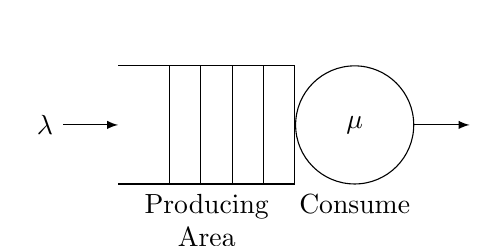
\begin{tikzpicture}[start chain=going right,>=latex,node distance=0pt]
		% the rectangular shape with vertical lines
		\node[rectangle split, rectangle split parts=6,
		draw, rectangle split horizontal,text height=1cm,text depth=0.5cm,on chain,inner ysep=0pt] (wa) {};
		\fill[white] ([xshift=-\pgflinewidth,yshift=-\pgflinewidth]wa.north west) rectangle ([xshift=-15pt,yshift=\pgflinewidth]wa.south);
		
		% the circle
		\node[draw,circle,on chain,minimum size=1.5cm] (se) {$\mu$};
		
		% the arrows and labels
		\draw[->] (se.east) -- +(20pt,0);
		\draw[<-] (wa.west) -- +(-20pt,0) node[left] {$\lambda$};
		\node[align=center,below] at (wa.south) {Producing \\ Area};
		\node[align=center,below] at (se.south) {Consume};
		\end{tikzpicture}
		\caption{a queue}
		\label{fig:queue0}
	\end{figure}
	
	\begin{figure}
		\centering
		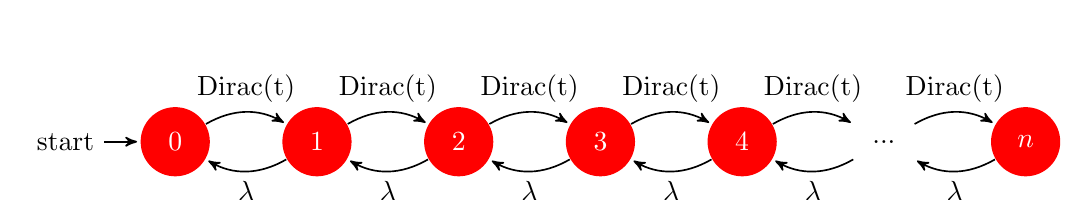
\begin{tikzpicture}[->,>=stealth',shorten >=1pt,auto,node distance=1.8cm,
		semithick]
		\tikzstyle{every state}=[fill=red,draw=none,text=white]
		
		\node[initial,state] (s0)                    {$0$};
		\node[state]         (s1) [right of=s0] {$1$};
		\node[state]         (s2) [right of=s1] {$2$};
		\node[state]         (s3) [right of=s2] {$3$};
		\node[state]         (s4) [right of=s3]       {$4$};
		\node[state]         (sw) [right of=s4,fill=white,text=black]       {...};
		\node[state]         (sn) [right of=sw]       {$n$};
		
		
		
		\path (s0) edge [bend left]             node {Dirac(t)} (s1)
		(s1) edge [bend left] node {$\lambda$} (s0)
		edge  [bend left]            node {Dirac(t)} (s2)
		(s2) edge [bend left]             node {$\lambda$} (s1)
		edge [bend left]  node {Dirac(t)} (s3)
		(s3) edge [bend left]              node {$\lambda$} (s2)
		edge [bend left]  node {Dirac(t)} (s4)
		(s4) edge [bend left]             node {$\lambda$} (s3)
		edge [bend left]  node {Dirac(t)} (sw)
		(sw) edge [bend left]             node {$\lambda$} (s4)
		edge [bend left]  node {Dirac(t)} (sn)
		(sn) edge [bend left]             node {$\lambda$} (sw);
		\end{tikzpicture}
		\caption{D/M/1/n queue with capacity $n$. The Dirac-distributed arrival event does not reset when the exponential service event occurs.}
		\label{fig:Queue1}
	\end{figure}
	
	\begin{figure}
		\centering
		\lstinputlisting{../Model/timeoutqueue.sm}

		\caption{PRISM GSMP model of a D/M/1/n queue as shown in \ref{fig:Queue1}.}
		\label{fig:queuecode1}
	\end{figure}
	
	%%%%%%%%%%%%%%%%%%%%%%%%%%%%%%%%%%%%%%%%%%%%%%%%%%%%%%%%%%%%%%%%%%%%%%%%%%%%%
	%%%%%%%%%%%%%%%%%%%%%%%%%%%%%%%%%SECTION2%%%%%%%%%%%%%%%%%%%%%%%%%%%%%%%%%%%%
	%%%%%%%%%%%%%%%%%%%%%%%%%%%%%%%%%%%%%%%%%%%%%%%%%%%%%%%%%%%%%%%%%%%%%%%%%%%%%
	
	\subsection{second model(using phase type fitting)}
	The timeout part is replaced by $k$ $\mu$ transition following the exponential law of parameter $\mu$. Here on the figure, k=5, which mean that you need 5 consecutive $\mu$ transition to $produce$. 
	
	
	\begin{figure}
		\centering
		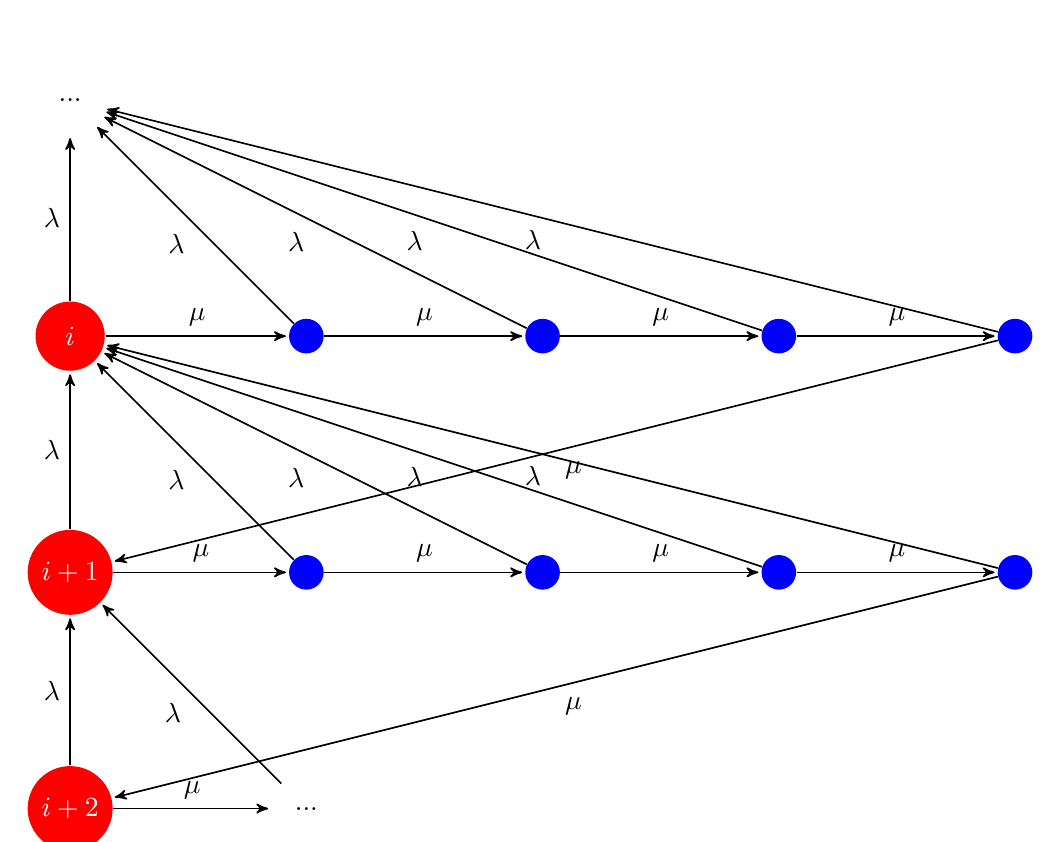
\begin{tikzpicture}[->,>=stealth',shorten >=1pt,auto,node distance=3.0cm,
		semithick]
		\tikzstyle{every state}=[fill=red,draw=none,text=white]
		
		\node[state] (s0)                    {$i$};
		\node[state] (s02) [right of=s0,fill=blue,scale=0.5]                   {};
		\node[state] (s03) [right of=s02,fill=blue,scale=0.5]                    {};
		\node[state] (s04) [right of=s03,fill=blue,scale=0.5]                   {};
		\node[state] (s05) [right of=s04,fill=blue,scale=0.5]                    {};
		\node[state] (s1) [below of=s0]                   {$i+1$};
		
		\node[state] (s12) [right of=s1,fill=blue,scale=0.5]                   {};
		\node[state] (s13) [right of=s12,fill=blue,scale=0.5]                    {};
		\node[state] (s14) [right of=s13,fill=blue,scale=0.5]                   {};
		\node[state] (s15) [right of=s14,fill=blue,scale=0.5]                    {};
		\node[state] (s2) [below of=s1]     {$i+2$};
		
		\node[state] (sw0) [above of=s0,fill=white,text=black]        {...}            {};
		\node[state] (sw1) [right of=s2,fill=white,text=black]       {...}             {};
		
		
		
		
		\path (s0) edge   node {$\lambda$} (sw0)
		edge   node {$\mu$} (s02)
		
		(s02)   edge   node {$\lambda$} (sw0)
		edge   node {$\mu$} (s03)
		(s03)   edge  node {$\lambda$} (sw0)
		edge   node {$\mu$} (s04)
		(s04) edge  node {$\lambda$} (sw0)
		edge   node {$\mu$} (s05)
		(s05) edge  node {$\lambda$} (sw0)
		edge   node {$\mu$} (s1)
		(s1)    edge  node {$\lambda$} (s0)
		edge   node {$\mu$} (s12)
		(s12)   edge  node {$\lambda$} (s0)
		edge   node {$\mu$} (s13)
		(s13) edge  node {$\lambda$} (s0)
		edge   node {$\mu$} (s14)
		(s14) edge  node {$\lambda$} (s0)
		edge   node {$\mu$} (s15)
		(s15) edge  node {$\lambda$} (s0)
		edge   node {$\mu$} (s2)
		(s2) edge  node {$\lambda$} (s1)
		edge   node {$\mu$} (sw1)    
		(sw1) edge  node {$\lambda$} (s1);
		\end{tikzpicture}
		\caption{Queue with phase type fitting of parameter k.}
		\label{fig:queueptf1}
	\end{figure}
	
	\begin{figure}
		\centering
		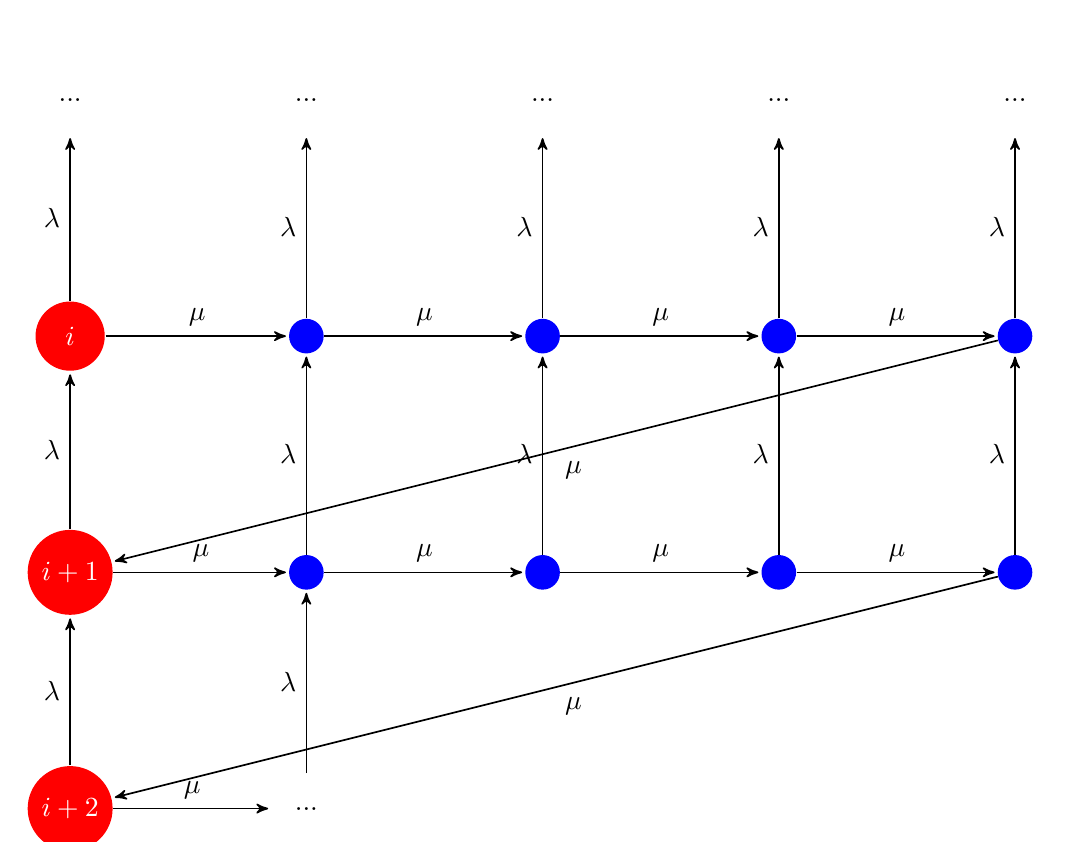
\begin{tikzpicture}[->,>=stealth',shorten >=1pt,auto,node distance=3.0cm,
		semithick]
		\tikzstyle{every state}=[fill=red,draw=none,text=white]
		
		\node[state] (s0)                    {$i$};
		\node[state] (s02) [right of=s0,fill=blue,scale=0.5]                   {};
		\node[state] (s03) [right of=s02,fill=blue,scale=0.5]                    {};
		\node[state] (s04) [right of=s03,fill=blue,scale=0.5]                   {};
		\node[state] (s05) [right of=s04,fill=blue,scale=0.5]                    {};
		\node[state] (s1) [below of=s0]                   {$i+1$};
		
		\node[state] (s12) [right of=s1,fill=blue,scale=0.5]                   {};
		\node[state] (s13) [right of=s12,fill=blue,scale=0.5]                    {};
		\node[state] (s14) [right of=s13,fill=blue,scale=0.5]                   {};
		\node[state] (s15) [right of=s14,fill=blue,scale=0.5]                    {};
		\node[state] (s2) [below of=s1]     {$i+2$};
		
		\node[state] (sw0) [above of=s0,fill=white,text=black]        {...}            {};
		\node[state] (sw02) [right of=sw0,fill=white,text=black]        {...}            {};
		\node[state] (sw03) [right of=sw02,fill=white,text=black]        {...}            {};
		\node[state] (sw04) [right of=sw03,fill=white,text=black]        {...}            {};
		\node[state] (sw05) [right of=sw04,fill=white,text=black]        {...}            {};
		\node[state] (sw1) [right of=s2,fill=white,text=black]       {...}             {};
		
		
		
		
		\path (s0) edge   node {$\lambda$} (sw0)
		edge   node {$\mu$} (s02)
		
		(s02)   edge   node {$\lambda$} (sw02)
		edge   node {$\mu$} (s03)
		(s03)   edge  node {$\lambda$} (sw03)
		edge   node {$\mu$} (s04)
		(s04) edge  node {$\lambda$} (sw04)
		edge   node {$\mu$} (s05)
		(s05) edge  node {$\lambda$} (sw05)
		edge   node {$\mu$} (s1)
		(s1)    edge  node {$\lambda$} (s0)
		edge   node {$\mu$} (s12)
		(s12)   edge  node {$\lambda$} (s02)
		edge   node {$\mu$} (s13)
		(s13) edge  node {$\lambda$} (s03)
		edge   node {$\mu$} (s14)
		(s14) edge  node {$\lambda$} (s04)
		edge   node {$\mu$} (s15)
		(s15) edge  node {$\lambda$} (s05)
		edge   node {$\mu$} (s2)
		(s2) edge  node {$\lambda$} (s1)
		edge   node {$\mu$} (sw1)    
		(sw1) edge  node {$\lambda$} (s12);
		\end{tikzpicture}
		\caption{Queue with phase type fitting of parameter k.}
		\label{fig:queueptf2}
	\end{figure}
	
	\begin{figure}
		\centering
		\begin{lstlisting}
		gsmp
		
		const int k = 10;
		const int qCapacity = 10;
		
		const double timeout = 10;
		const double lambda = 0.2;
		
		
		
		module main
		
		qSize : [0..qCapacity] init 0;
		
		[produce] (qSize < qCapacity) -> (qSize' = qSize+1);
		[consume] (qSize > 0) -> lambda: (qSize' = qSize - 1);
		
		endmodule
		
		module trigger
		
		i : [1..k+1];
		
		[] i < k -> k/timeout : (i'=i+1);
		[produce] i = k -> k/timeout : (i'=1);
		//[consume] true -> (i'=1);
		
		endmodule
		
		\end{lstlisting}
		\caption{PRISM CTMC model of the D/M/1/n queue as shown in \ref{fig:Queue1} with phase-type fitting to approximate the deterministic arrivals. The phase-type module \emph{trigger} is used as suggested on the \href{http://www.prismmodelchecker.org/manual/FrequentlyAskedQuestions/PRISMModelling}{PRISM website}.  }
		\label{fig:queuecode2}
	\end{figure}
	
	\begin{figure}
		\centering
		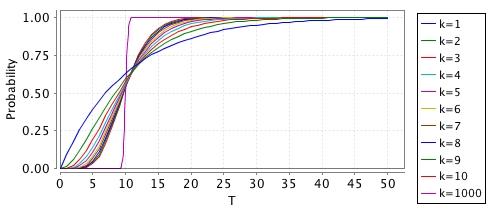
\includegraphics[width=12cm]{faq-erlang.jpg}
		\caption{The effect of $k$, the number of time points within the sequence of exponential transitions, on the shape of the resulting phase-type distribution. Increasing $k$ makes the phase-type distribution more deterministic. This picture was taken from the \href{http://www.prismmodelchecker.org/manual/FrequentlyAskedQuestions/PRISMModelling}{PRISM website}.}
		\label{fig:time1}
	\end{figure}
	
	
	
	
	\subsection{finding $\mu$}
	
	According to Prism documentation on phase type fittimg, we should take $\mu = t/k$. The mean of diract(t) is t, and the mean of exponential($\mu$) is $1/\mu$. Hence $\mu = t/k$.
	
	
	
	\subsection{Results}
	
	For a queue capacity of 10, we compare the steady state probabilities according to k the parameter of phase type fitting.
	
	\begin{figure}
		\centering
		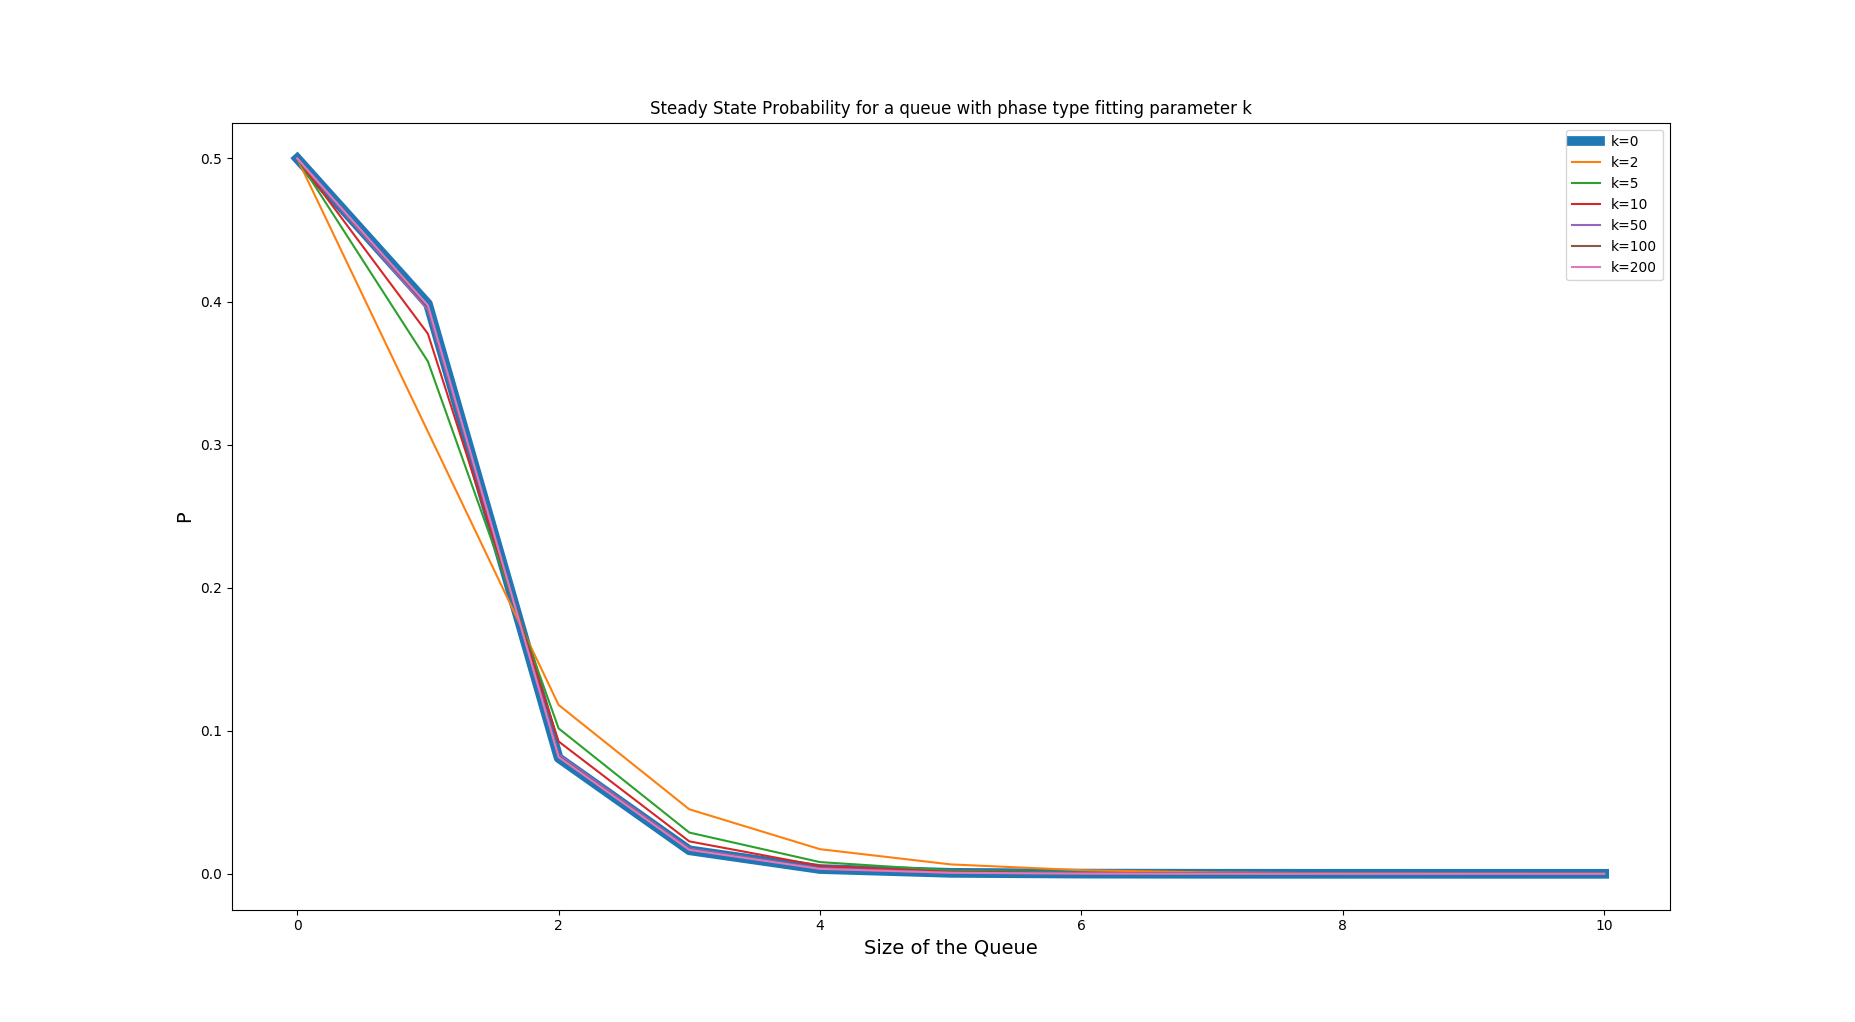
\includegraphics[width=18cm]{sspqueue.png}
		\caption{The blue line is the result without phase type fitting.}
		\label{fig:res1}
	\end{figure}
	
	\begin{figure}
		\centering
		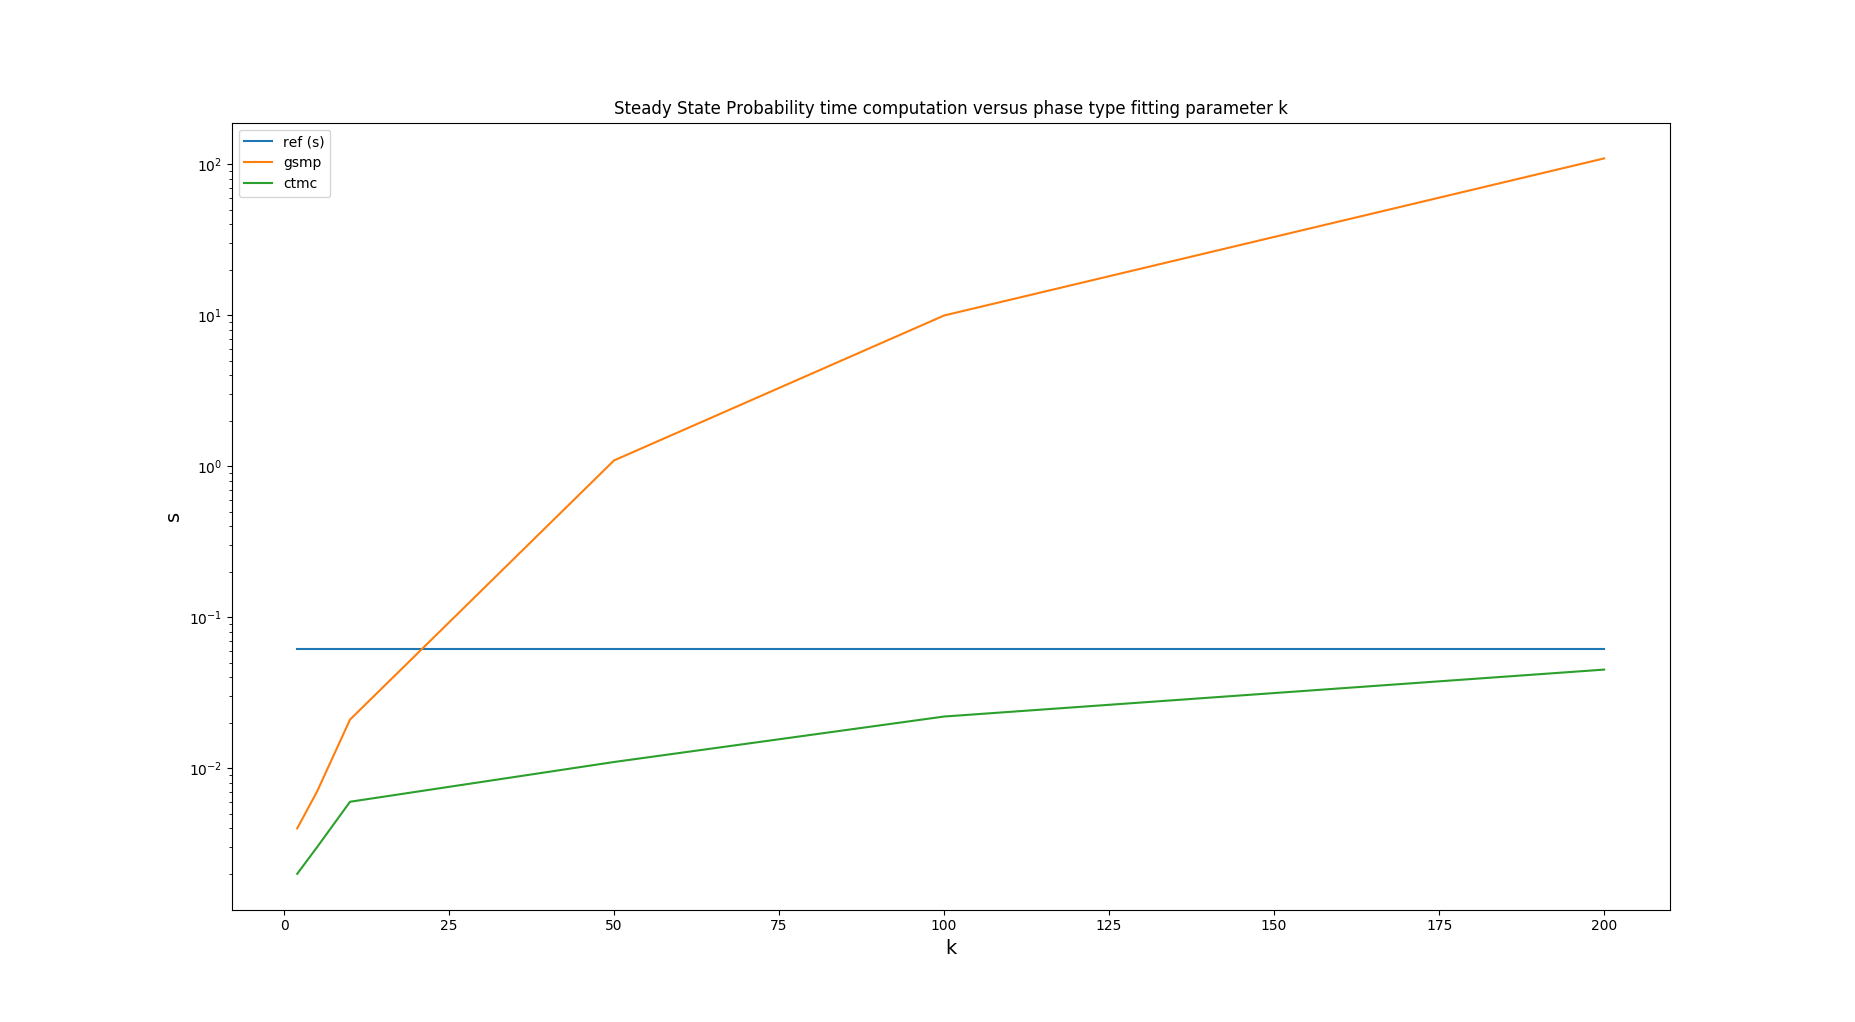
\includegraphics[width=16cm]{time.png}
		\caption{Computation time for different values of $k$. The growing lines represent computations of models with phase-type distributions. For about $k>200$, GSMP implementation starts outperforming all phase-typed computations, despite the GSMP implementation being relatively poorly optimized.}
		\label{fig:time1}
	\end{figure}	
	
	\begin{figure}
		\centering
		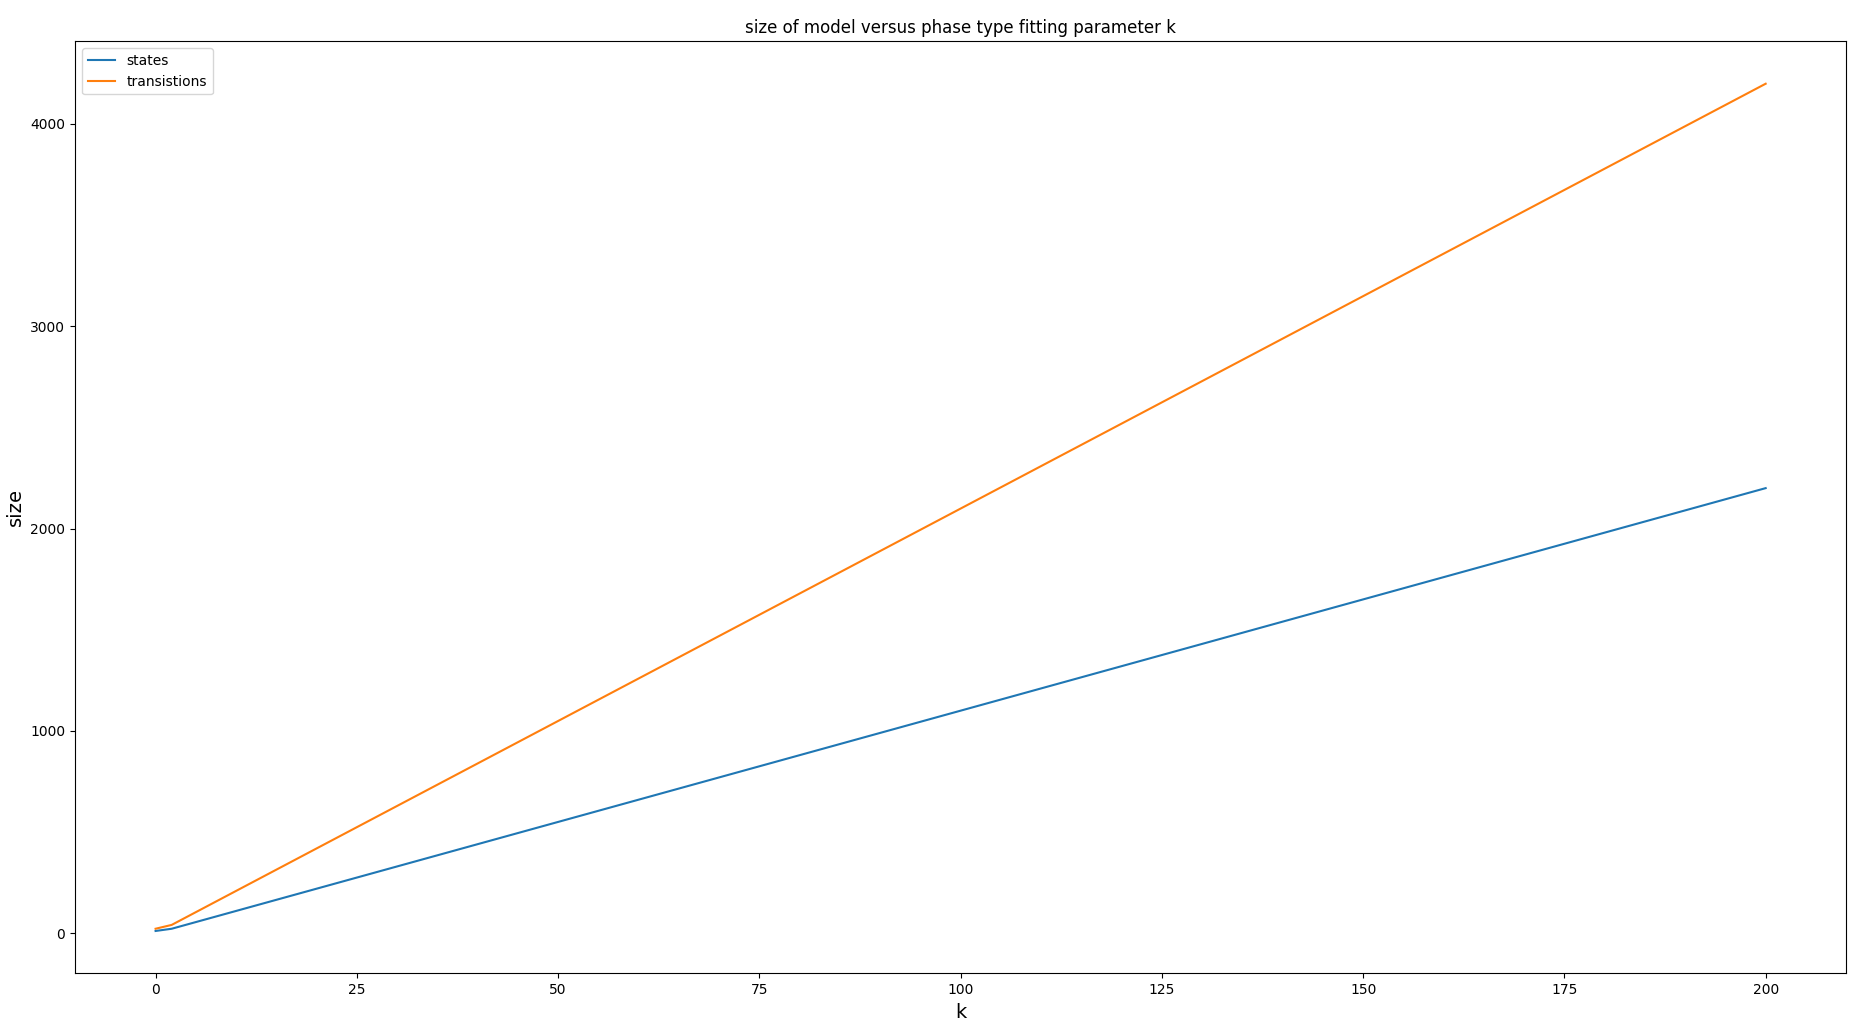
\includegraphics[width=16cm]{size.png}
		\caption{Size of model for different values of $k$.}
		\label{fig:time1}
	\end{figure}

	
	\subsubsection{parameters}

	\begin{figure}
		\centering
		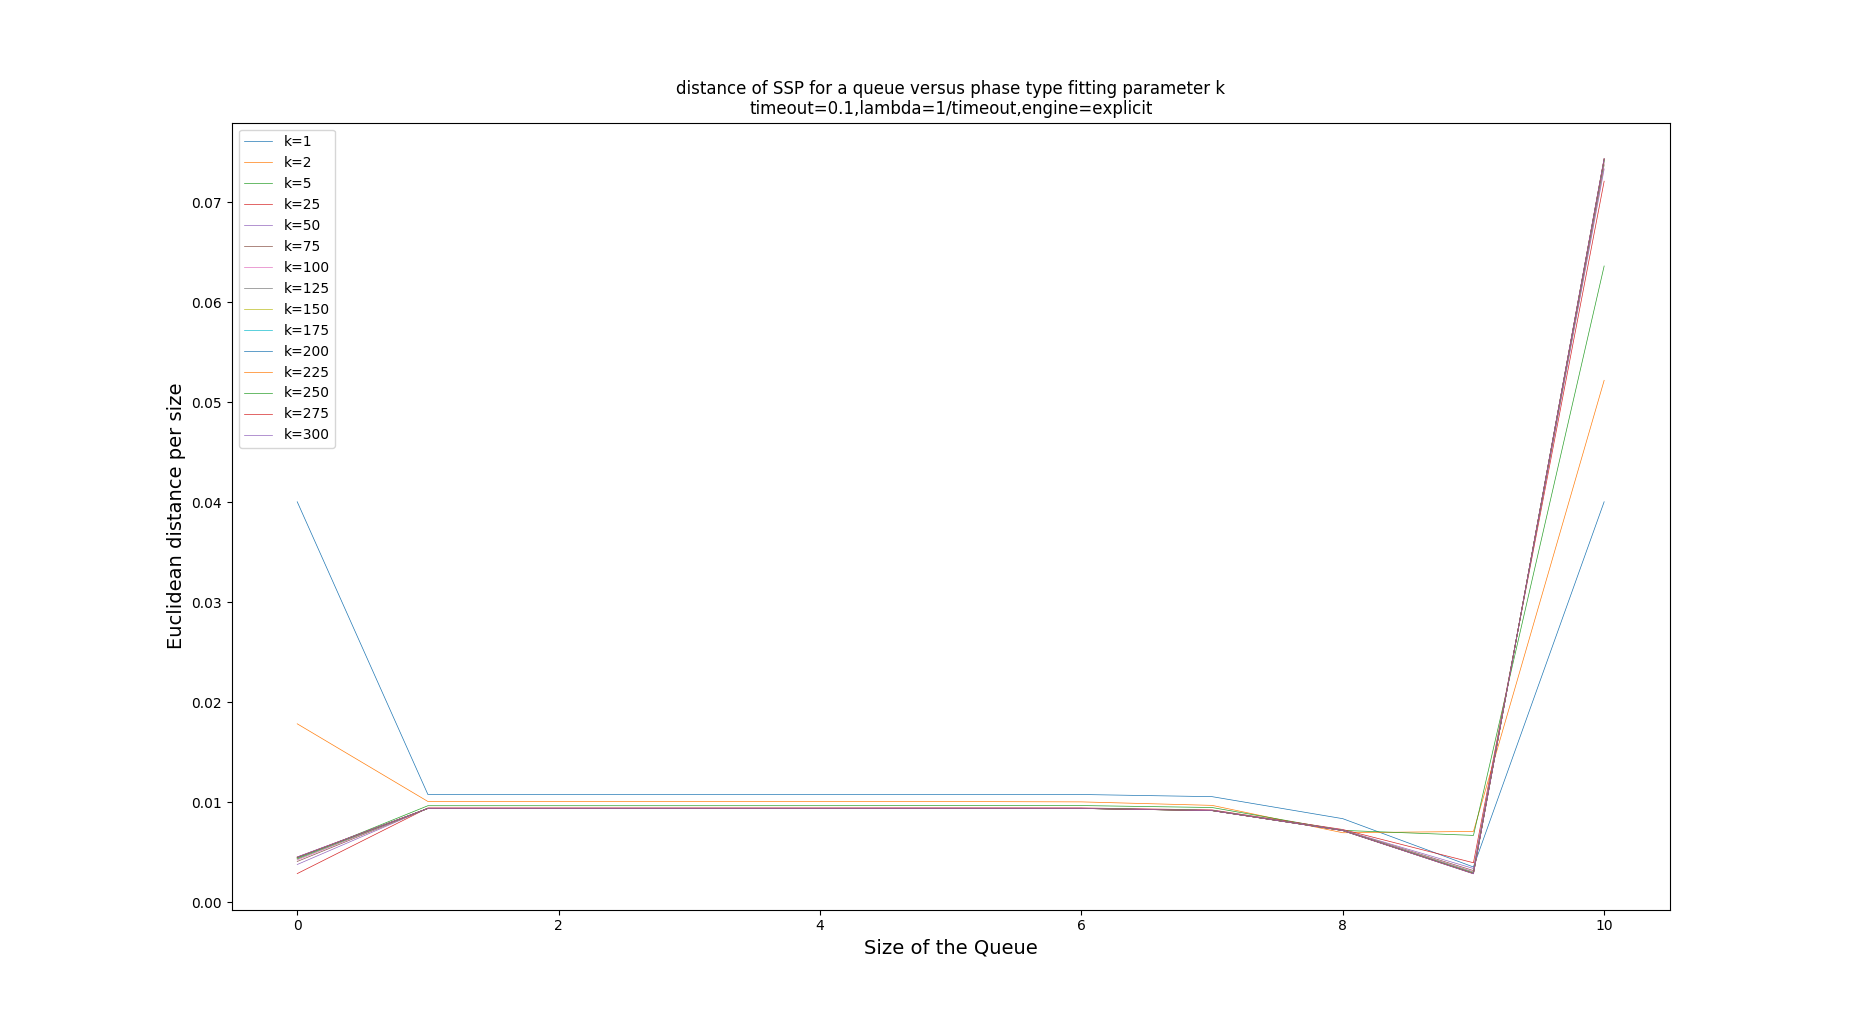
\includegraphics[width=18cm]{diff_explicit_01.png}
		\caption{Distance of result of the SSP computation between the event model and the PTF model using explicit engine,	$t=0.1$,$\lambda=1/t$,$\epsilon=10^{-5}$}
		\label{fig:diff_explicit_01}
	\end{figure}

	\begin{figure}
		\centering
		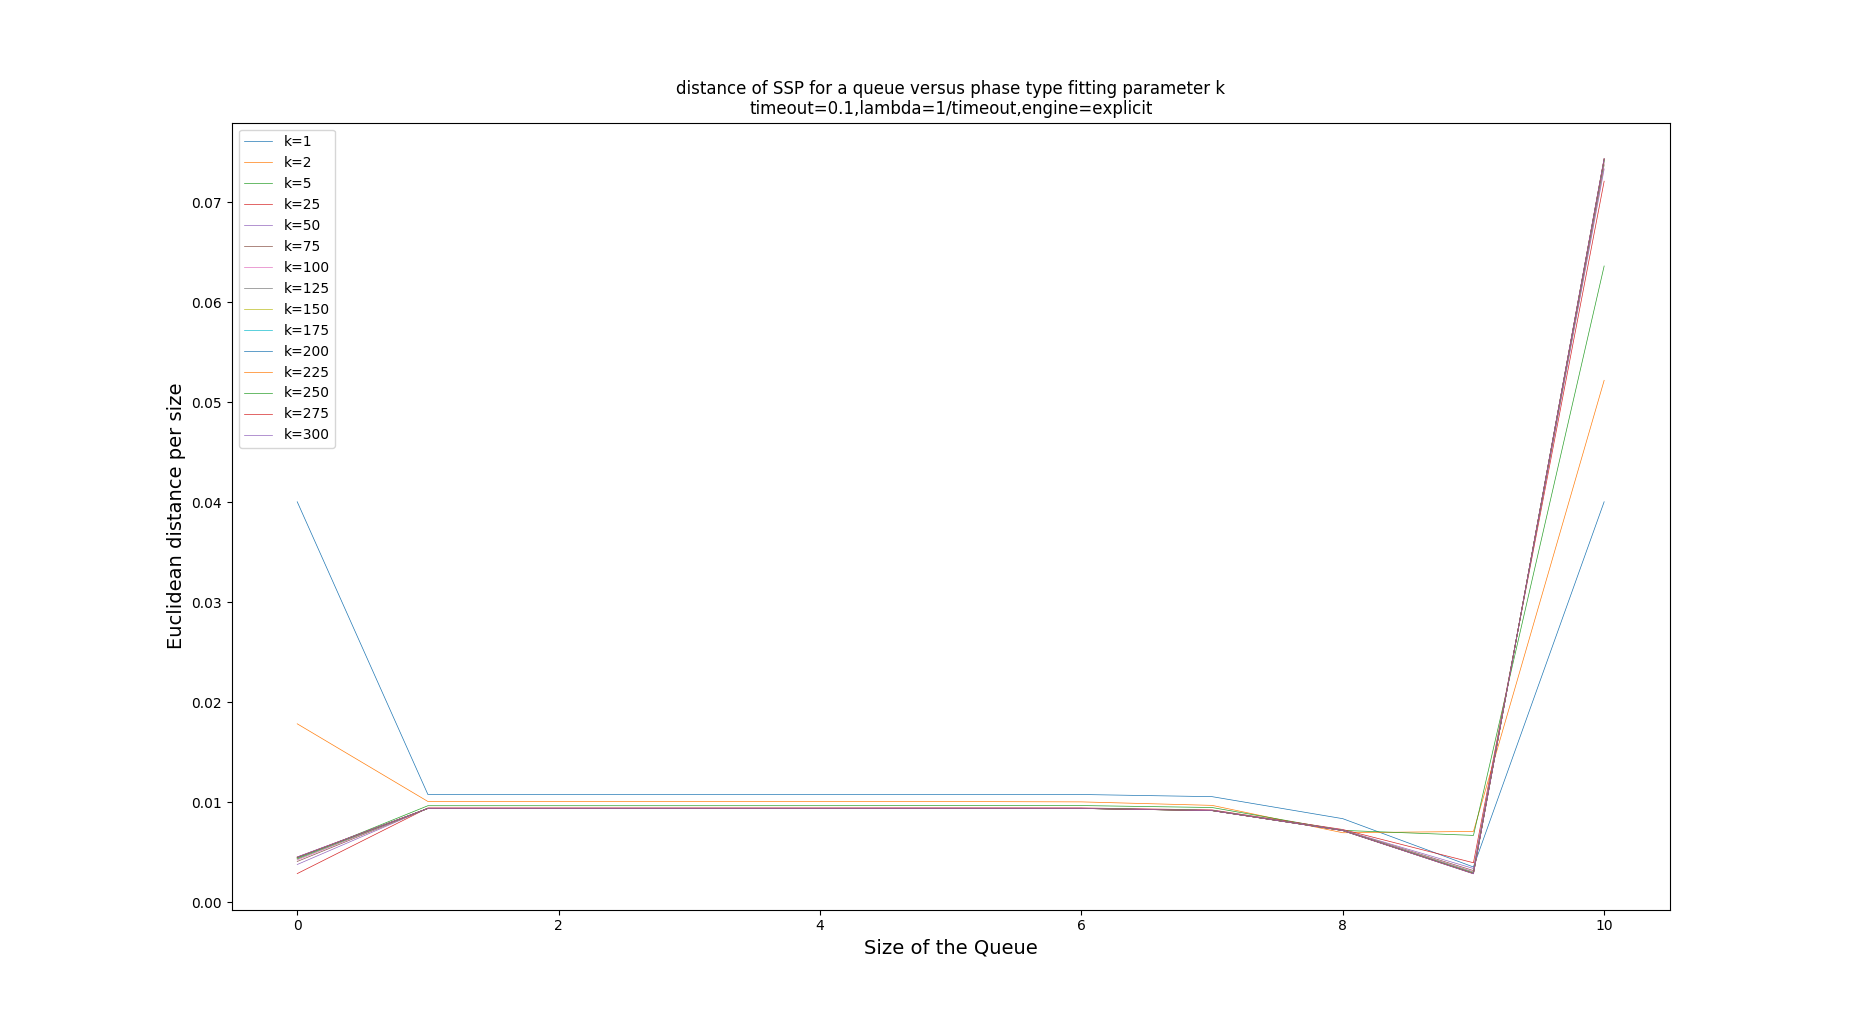
\includegraphics[width=18cm]{diff_explicit_01.png}
		\caption{Distance of result of the SSP computation between the event model and the PTF model using hybrid engine,	$t=0.1$,$\lambda=1/t$,$\epsilon=10^{-5}$}
		\label{fig:diff_hybrid_01}
	\end{figure}
	
	\begin{figure}
		\centering
		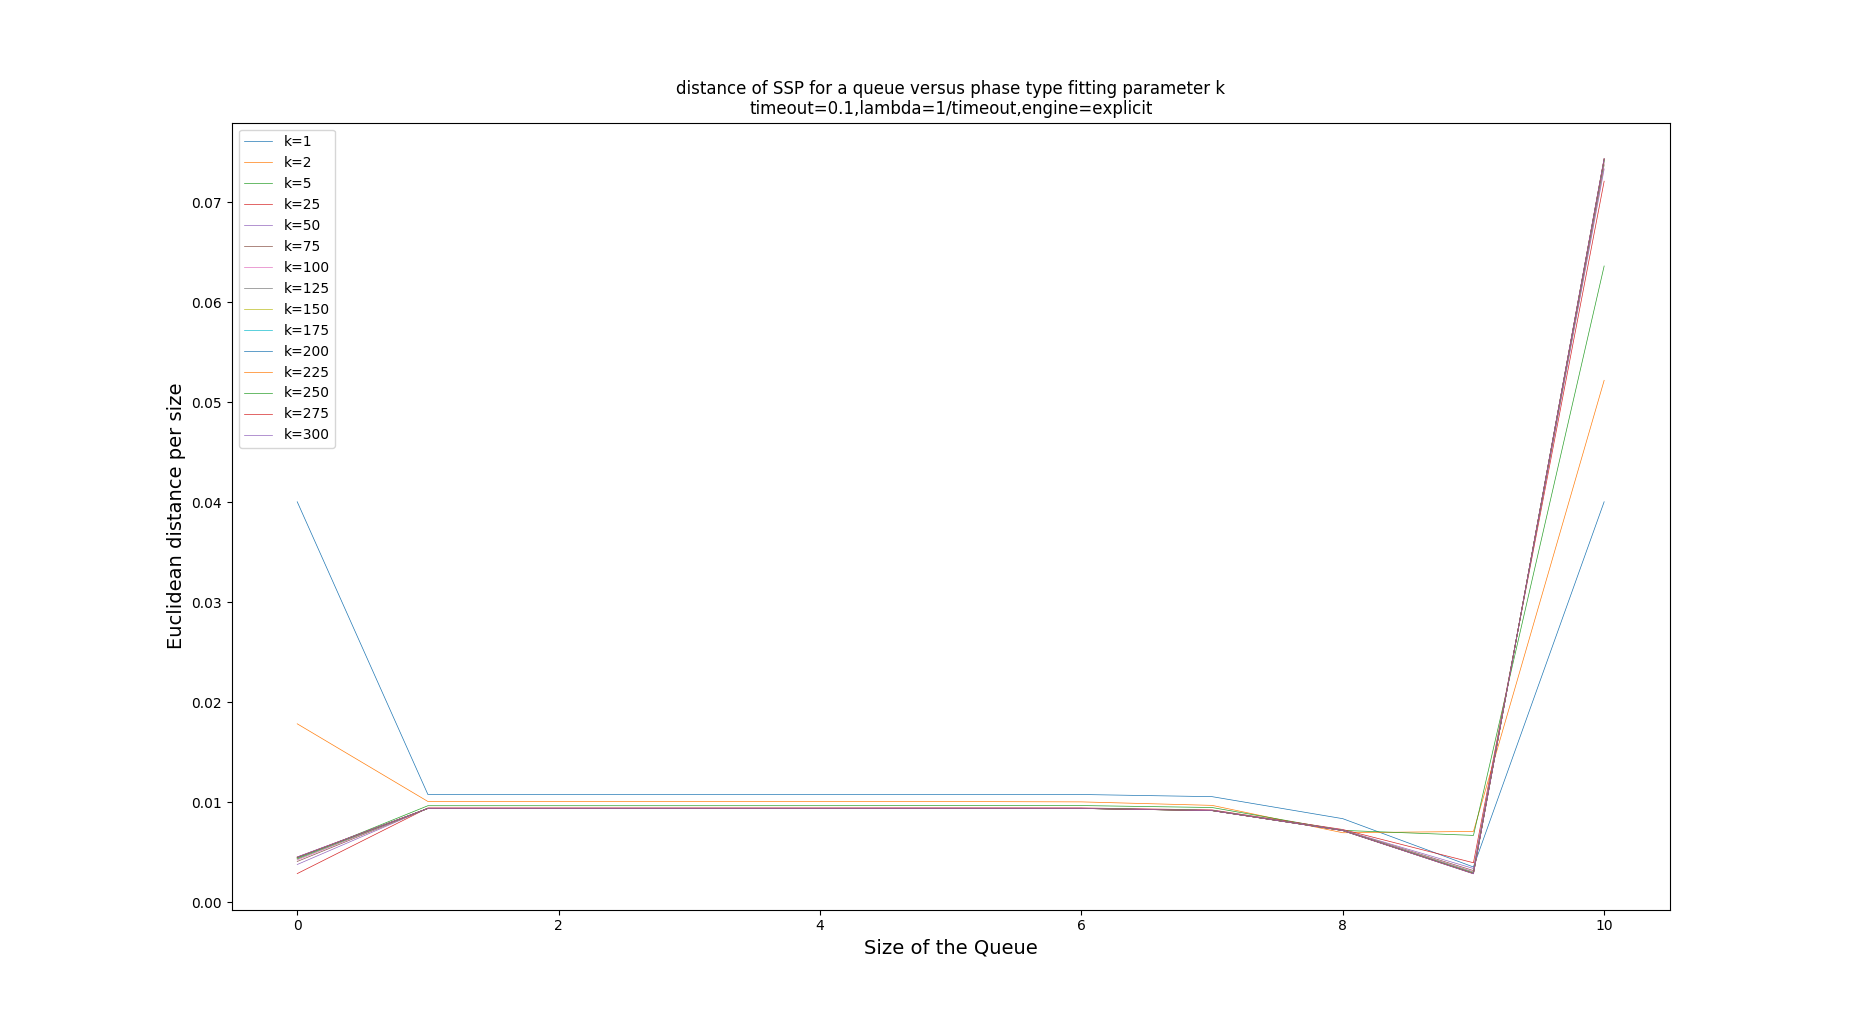
\includegraphics[width=18cm]{diff_explicit_01.png}
		\caption{Distance of result of the SSP computation between the event model and the PTF model using explicit engine,	$t=0.1$,$\lambda=1/t$,$\epsilon=10^{-5}$}
		\label{fig:diff_explicit_001}
	\end{figure}


	%%% End document
\end{document}\\

